\documentclass{article}

\usepackage{tikz}
\usetikzlibrary{spath3}

\begin{document}

\section{Original Paths}

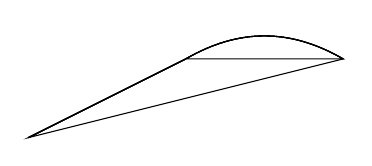
\begin{tikzpicture}
\draw[spath/show current path] (0,0) -- (2,1);
\draw[spath/show current path] (0,0) -- (2,1) to[out=30, in=150] +(2,0);
\draw[spath/show current path] (0,0) -- (2,1) +(0,0) to[out=30, in=150] +(2,0);
\draw[spath/show current path] (0,0) -- (2,1) to[out=30, in=150] +(2,0) -- cycle;
\draw[spath/show current path] (0,0) -- (2,1) +(0,0) to[out=30, in=150] +(2,0) -- cycle;
\end{tikzpicture}

\section{Reversed Paths}

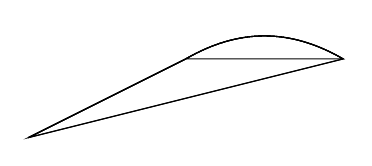
\begin{tikzpicture}
\draw[spath/show current path] (2,1) -- (0,0);
\draw[spath/show current path] (4,1) to[out=150,in=30] +(-2,0) -- (0,0);
\draw[spath/show current path] (4,1) to[out=150,in=30] +(-2,0) +(0,0) -- (0,0);
\draw[spath/show current path] (4,1) to[out=150,in=30] +(-2,0) -- (0,0) -- cycle;
\draw[spath/show current path] (4,1) to[out=150,in=30] +(-2,0) -- cycle (2,1) -- (0,0);
\end{tikzpicture}

\section{Translated Paths}

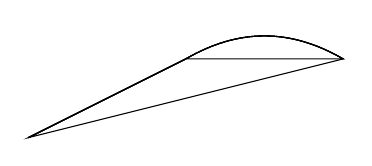
\begin{tikzpicture}
\begin{scope}[shift={(2,3)}]
\draw[spath/show current path] (0,0) -- (2,1);
\draw[spath/show current path] (0,0) -- (2,1) to[out=30, in=150] +(2,0);
\draw[spath/show current path] (0,0) -- (2,1) +(0,0) to[out=30, in=150] +(2,0);
\draw[spath/show current path] (0,0) -- (2,1) to[out=30, in=150] +(2,0) -- cycle;
\draw[spath/show current path] (0,0) -- (2,1) +(0,0) to[out=30, in=150] +(2,0) -- cycle;
\end{scope}

\end{tikzpicture}

\section{Scaled Paths}

\begin{tikzpicture}
\begin{scope}[xscale=5, yscale=2]
\draw[spath/show current path] (0,0) -- (2,1);
\draw[spath/show current path] (0,0) -- (2,1) to[out=30, in=150] +(2,0);
\draw[spath/show current path] (0,0) -- (2,1) +(0,0) to[out=30, in=150] +(2,0);
\draw[spath/show current path] (0,0) -- (2,1) to[out=30, in=150] +(2,0) -- cycle;
\draw[spath/show current path] (0,0) -- (2,1) +(0,0) to[out=30, in=150] +(2,0) -- cycle;
\end{scope}

\end{tikzpicture}

\section{Transformed Paths}

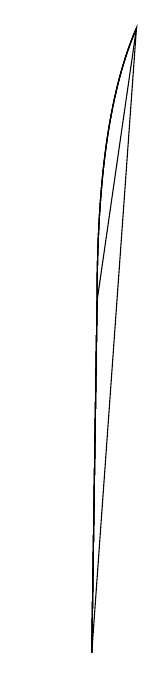
\begin{tikzpicture}
\begin{scope}[xscale=.5, yscale=2, rotate=60, shift={(-2,-3)}]
\draw[spath/show current path] (0,0) -- (2,1);
\draw[spath/show current path] (0,0) -- (2,1) to[out=30, in=150] +(2,0);
\draw[spath/show current path] (0,0) -- (2,1) +(0,0) to[out=30, in=150] +(2,0);
\draw[spath/show current path] (0,0) -- (2,1) to[out=30, in=150] +(2,0) -- cycle;
\draw[spath/show current path] (0,0) -- (2,1) +(0,0) to[out=30, in=150] +(2,0) -- cycle;
\path[spath/show current path] (0,0) (1,0) (0,1);
\end{scope}
\begin{scope}[xscale=.5, yscale=2, rotate=60]
\path[spath/show current path] (0,0) (1pt,0) (0,1pt);
\end{scope}
\end{tikzpicture}

\section{welded Paths}

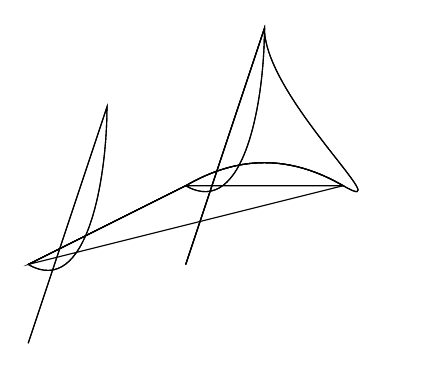
\begin{tikzpicture}
\draw[spath/show current path] (0,0) to[out=-30,in=-90] ++(1,2) -- ++(-1,-3);
\draw[spath/show current path] (0,0) -- (2,1) to[out=-30,in=-90] ++(1,2) -- ++(-1,-3);
\draw[spath/show current path] (0,0) -- (2,1) to[out=30, in=150] +(2,0) to[out=-30,in=-90] ++(1,2) -- ++(-1,-3);
\draw[spath/show current path] (0,0) -- (2,1) +(0,0) to[out=30, in=150] +(2,0) to[out=-30,in=-90] ++(1,2) -- ++(-1,-3);
\draw[spath/show current path] (0,0) -- (2,1) to[out=30, in=150] +(2,0) -- cycle to[out=-30,in=-90] ++(1,2) -- ++(-1,-3);
\draw[spath/show current path] (0,0) -- (2,1) +(0,0) to[out=30, in=150] +(2,0) -- cycle to[out=-30,in=-90] ++(1,2) -- ++(-1,-3);
\end{tikzpicture}

\section{Appended Paths, No Move}

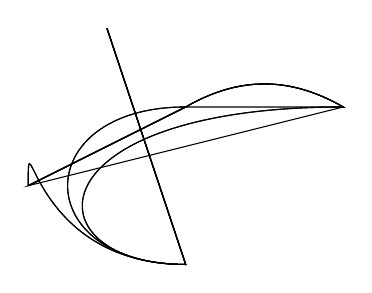
\begin{tikzpicture}
\draw[spath/show current path] (0,0) .. controls (0,1) and (0,-1) .. (2,-1) -- (1,2);
\draw[spath/show current path] (0,0) -- (2,1) .. controls (0,1) and (0,-1) .. (2,-1) -- (1,2);
\draw[spath/show current path] (0,0) -- (2,1) to[out=30, in=150] +(2,0) .. controls (0,1) and (0,-1) .. (2,-1) -- (1,2);
\draw[spath/show current path] (0,0) -- (2,1) +(0,0) to[out=30, in=150] +(2,0) .. controls (0,1) and (0,-1) .. (2,-1) -- (1,2);
\draw[spath/show current path] (0,0) -- (2,1) to[out=30, in=150] +(2,0) -- cycle .. controls (0,1) and (0,-1) .. (2,-1) -- (1,2);
\draw[spath/show current path] (0,0) -- (2,1) +(0,0) to[out=30, in=150] +(2,0) -- cycle .. controls (0,1) and (0,-1) .. (2,-1) -- (1,2);
\end{tikzpicture}

\section{Appended Paths}

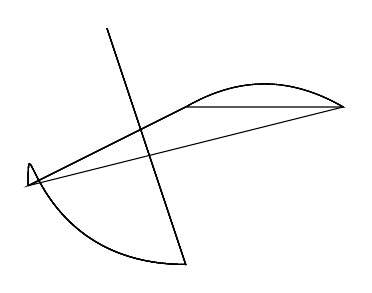
\begin{tikzpicture}
\draw[spath/show current path] (0,0) .. controls (0,1) and (0,-1) .. (2,-1) -- (1,2);
\draw[spath/show current path] (0,0) -- (2,1) (0,0) .. controls (0,1) and (0,-1) .. (2,-1) -- (1,2);
\draw[spath/show current path] (0,0) -- (2,1) to[out=30, in=150] +(2,0) (0,0) .. controls (0,1) and (0,-1) .. (2,-1) -- (1,2);
\draw[spath/show current path] (0,0) -- (2,1) +(0,0) to[out=30, in=150] +(2,0) (0,0) .. controls (0,1) and (0,-1) .. (2,-1) -- (1,2);
\draw[spath/show current path] (0,0) -- (2,1) to[out=30, in=150] +(2,0) -- cycle (0,0) .. controls (0,1) and (0,-1) .. (2,-1) -- (1,2);
\draw[spath/show current path] (0,0) -- (2,1) +(0,0) to[out=30, in=150] +(2,0) -- cycle (0,0) .. controls (0,1) and (0,-1) .. (2,-1) -- (1,2);
\end{tikzpicture}

\section{Intersection Components}

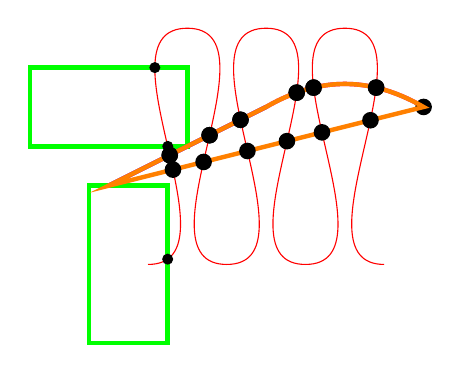
\begin{tikzpicture}
\draw[spath/show current path] (0,0) -- (2,1);
\draw[spath/show current path] (.75,-2) rectangle ++(-1,2);
\draw[spath/show current path] (-1,.5) rectangle ++(2,1);
\draw[spath/show current path] (0,0) -- (2,1) to[out=30, in=150] +(2,0);
\draw[spath/show current path] (0,0) -- (2,1) to[out=30, in=150] +(2,0) -- cycle;
\draw[spath/show current path, red] (.5,-1) to[out=0,in=180] ++(.5,3) to[out=0,in=180] ++(.5,-3) to[out=0,in=180] ++(.5,3) to[out=0,in=180] ++(.5,-3) to[out=0,in=180] ++(.5,3) to[out=0,in=180] ++(.5,-3)
;

\draw[ultra thick, blue]
(0.0pt,0.0pt) --
(22.0895731082pt,11.0447846132pt)
(22.0895731082pt,11.0447846132pt) --
(36.4826786939pt,18.2413361414pt)
(36.4826786939pt,18.2413361414pt) --
(47.652657326pt,23.826324476pt)
(47.652657326pt,23.826324476pt) --
(56.90549pt,28.45274pt)
;

\fill
(22.0895731082pt,11.0447846132pt) circle[radius=2pt]
(36.4826786939pt,18.2413361414pt) circle[radius=2pt]
(47.652657326pt,23.826324476pt) circle[radius=2pt]
;


\draw[ultra thick, green]
(21.33955pt,-26.5355990419pt) --
(21.33955pt,0.0pt) --
(-7.11319pt,0.0pt) --
(-7.11319pt,-56.90549pt) --
(21.33955pt,-56.90549pt) --
(21.33955pt,-26.5355990419pt)
;

\draw[ultra thick, green]
(16.6994821608pt,42.67911pt) --
(28.45274pt,42.67911pt) --
(28.45274pt,14.22636pt) --
(21.3674386852pt,14.22636pt)
(21.3674386852pt,14.22636pt) --
(-28.45274pt,14.22636pt) --
(-28.45274pt,42.67911pt) --
(16.6994821608pt,42.67911pt)
;

\fill
(21.33955pt,-26.5355990419pt) circle[radius=2pt]
(21.3674386852pt,14.22636pt) circle[radius=2pt]
(16.6994821608pt,42.67911pt) circle[radius=2pt]
;

\draw[ultra thick, magenta]
(0.0pt,0.0pt) --
(22.0895731082pt,11.0447846132pt)
(22.0895731082pt,11.0447846132pt) --
(36.4826786939pt,18.2413361414pt)
(36.4826786939pt,18.2413361414pt) --
(47.652657326pt,23.826324476pt)
(47.652657326pt,23.826324476pt) --
(56.90549pt,28.45274pt) .. controls 
(60.61213895060001pt,30.5927695877pt) and 
(64.29090142112955pt,32.32005166882031pt) .. 
(67.95253434241103pt,33.63458624336091pt)
(67.95253434241103pt,33.63458624336091pt) .. controls 
(69.99209064838535pt,34.36679161144769pt) and 
(72.02633238933044pt,34.97093911691348pt) .. 
(74.05711852959721pt,35.4470287597583pt)
(74.05711852959721pt,35.4470287597583pt) .. controls 
(81.60711373040281pt,37.21702041341389pt) and 
(89.10934626959721pt,37.2170204134139pt) .. 
(96.6593414704028pt,35.4470287597583pt)
(96.6593414704028pt,35.4470287597583pt) .. controls 
(102.3360153782694pt,34.1162112995861pt) and 
(108.039690486pt,31.784781713pt) .. 
(113.81097pt,28.45274pt)
;

\fill
(22.0895731082pt,11.0447846132pt) circle[radius=3pt]
(36.4826786939pt,18.2413361414pt) circle[radius=3pt]
(47.652657326pt,23.826324476pt) circle[radius=3pt]
(67.95253434241103pt,33.63458624336091pt) circle[radius=3pt]
(74.05711852959721pt,35.4470287597583pt) circle[radius=3pt]
(96.6593414704028pt,35.4470287597583pt) circle[radius=3pt]
(113.81097pt,28.45274pt) circle[radius=3pt]
;

\draw[ultra thick, orange, spath/show current path]
(22.0895731082pt,11.0447846132pt) --
(36.4826786939pt,18.2413361414pt)
(36.4826786939pt,18.2413361414pt) --
(47.652657326pt,23.826324476pt)
(47.652657326pt,23.826324476pt) --
(56.90549pt,28.45274pt) .. controls 
(60.61213895060001pt,30.5927695877pt) and 
(64.29090142112955pt,32.32005166882031pt) .. 
(67.95253434241103pt,33.63458624336091pt)
(67.95253434241103pt,33.63458624336091pt) .. controls 
(69.99209064838535pt,34.36679161144769pt) and 
(72.02633238933044pt,34.97093911691348pt) .. 
(74.05711852959721pt,35.4470287597583pt)
(74.05711852959721pt,35.4470287597583pt) .. controls 
(81.60711373040281pt,37.21702041341389pt) and 
(89.10934626959721pt,37.2170204134139pt) .. 
(96.6593414704028pt,35.4470287597583pt)
(96.6593414704028pt,35.4470287597583pt) .. controls 
(102.3360153782694pt,34.1162112995861pt) and 
(108.039690486pt,31.784781713pt) .. 
(113.81097pt,28.45274pt) --
(94.61105936100003pt,23.652762762pt)
(94.61105936100003pt,23.652762762pt) --
(77.10579406530003pt,19.2764468226pt)
(77.10579406530003pt,19.2764468226pt) --
(64.43521877520001pt,16.1088032784pt)
(64.43521877520001pt,16.1088032784pt) --
(50.15308014989997pt,12.53826893579999pt)
(50.15308014989997pt,12.53826893579999pt) --
(34.31514556469996pt,8.57878563739999pt)
(34.31514556469996pt,8.57878563739999pt) --
(23.2572717195pt,5.814317419pt)
(23.2572717195pt,5.814317419pt) --
(0.0pt,0.0pt) -- (22.0895731082pt,11.0447846132pt)
;

\fill
(36.4826786939pt,18.2413361414pt) circle[radius=3pt]
(47.652657326pt,23.826324476pt) circle[radius=3pt]
(67.95253434241103pt,33.63458624336091pt) circle[radius=3pt]
(74.05711852959721pt,35.4470287597583pt) circle[radius=3pt]
(96.6593414704028pt,35.4470287597583pt) circle[radius=3pt]
(94.61105936100003pt,23.652762762pt) circle[radius=3pt]
(77.10579406530003pt,19.2764468226pt) circle[radius=3pt]
(64.43521877520001pt,16.1088032784pt) circle[radius=3pt]
(50.15308014989997pt,12.53826893579999pt) circle[radius=3pt]
(34.31514556469996pt,8.57878563739999pt) circle[radius=3pt]
(23.2572717195pt,5.814317419pt) circle[radius=3pt]
(22.0895731082pt,11.0447846132pt) circle[radius=3pt]
;


\end{tikzpicture}

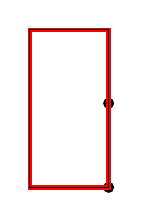
\begin{tikzpicture}

\fill
(21.33955pt, -26.5355990419pt) circle[radius=2pt]
(21.33955pt, -56.90549pt) circle[radius=2pt]
;

\draw[ultra thick, red]
(21.33955pt, -26.5355990419pt) -- 
(21.33955pt, 0.0pt) -- 
(-7.11319pt, 0.0pt) -- 
(-7.11319pt, -56.90549pt) -- 
(21.33955pt, -56.90549pt) -- 
(21.33955pt, -26.5355990419pt)
;


\draw
(21.33955pt, -56.90549pt) -- 
(21.33955pt, -26.5355990419pt)
(21.33955pt, -26.5355990419pt) -- 
(21.33955pt, 0.0pt) -- 
(-7.11319pt, 0.0pt) -- 
(-7.11319pt, -56.90549pt) -- 
(21.33955pt, -56.90549pt)
;
\end{tikzpicture}

\end{document}
